\FloatBarrier

\subsection{NEAREST KIFMM Hybrid} \label{sec:Hybrid}
The advantage of the KIFMM method comes from its fast approximation of distant source points, while NEAREST leverages the differences in the rate of change of the single-layer stokeslet kernel to approximate the kernel across the whole domain with fewer source points. If these methods were to be combined it would allow for an even more efficient approximation of source points in the far field and an improvement in near field calculations. Given that the reduction in source points is enough to create a smaller octtree, particularly when a non-adaptive tree is used, the KIFMM method should be able to compute the matrix problem in a shorter period of time. The adaption of the KIFMM method to use the nearest neighbour interpolation is a simple but fundamental change to the algorithm. When creating the octtree decomposition of the domain we form the tree based on target points and coarse source discretization as we would normally do. We then also generate the nearest neighbour interpolation matrix $\nu$ defined in \cref{eq:NNMatrix} between the coarse source points and the fine quadrature rule.  

In the upwards pass when calculating the upwards equivalent potential we replace the right-hand side of \cref{eq:upsum} with the nearest neighbour interpolation
\begin{equation*}
    \sum_{{\bm{y}}_{n} \in B} \bm{f}_{n}({\bm{y}}_n) \sum_{q=1}^{Q^*}S^{\epsilon}\left({\bm{q}}^{BD}_{k}, {\bm{X}}_{q}\right) \nu^*[q,n]
\end{equation*}
We define $\nu^*[q,n]$ as the subset of the full nearest neighbour matrix $\nu[q,n]$ corresponding to the map between points ${\bm{X}}_{q}$, and ${\bm{y}}_{n} \in B$. $Q^*$ is the number of fine quadrature points that map to ${\bm{y}}_{n} \in B$. This method provided an accurate approximation of the source points on the upward equivalent surfaces. The use of nearest neighbour interpolation in both the M2M translation (eq.~\ref{eq:M2M}) and the M2L translation (eq.~\ref{eq:M2L}) is not considered due to the need to compute the nearest neighbour matrix between all boxes. While the interactions between boxes are computed during the octtree generation and matrices could be precomputed, the number and size of these matrices make it inefficient to compute beforehand, particularly when nodes with small numbers of source points are considered. 
In the downwards pass we can also implement nearest neighbour interpolation when looking at the interaction lists of a node $B$, both $I_X^B$ and $I_U^B$ consider the point to point interactions directly due to them being in $\mathcal{N}(B)$. These translations are done through \cref{eq:X,eq:U} respectively. We now replace The right-hand side with 
\begin{equation*}
    \sum_{A_i \in I_X^B} \sum_{{\bm{y}}_n\in A_i} {\bm{f}}_{n} \sum_{q=1}^{Q^*} S^\epsilon\left(\bm{q}^{BU}_{k}, {\bm{X}}_{q}\right) \nu^*[q,n], \quad k=1,\dots,N_q
\end{equation*}
and
\begin{equation*}
    \sum_{{\bm{y}}_n\in A}{\bm{f}}_n \sum_{q=1}^{Q^*} S^\epsilon(\bm{x},{\bm{X}}_q) \nu^*[q,n]
\end{equation*}
respectively. Where $\nu^*[q,n]$ again corresponds to a slice of $\nu[q,n]$ which contains the respective map between source points and fine quadrature points in each summation.

As we considered in \cref{fig:NEARESTCOMP} we compute the relative residual error found by the hybrid KIFMM NEAREST method. As seen in \cref{fig:NEARESTCOMPFMM} the computed values mirror that found through the NEAREST method directly, with our implementation retaining the epsilon independence we see in the standard matrix formulation. We do note that the overall computation time of some of the resistance problems took longer than solving using the \textit{mldivide} operator on (M2) using \textit{gpuArrays}. This is due to the ill-conditioning of the NEAREST matrix for large values of $\epsilon$ as seen in \cref{appendix:ConNum}, particularly in the disjoint case. Preconditioning using a block-diagonal preconditioner described in \cref{sec:Preconditioning} can help reduce the overall number of GMRES but the calculation of the preconditioner means the overall computation time remains similar for resistance problems involving large $\epsilon$ values. 

\begin{figure}[ht!]
 \centering
 \subfloat[\label{fig:DISFMM}]{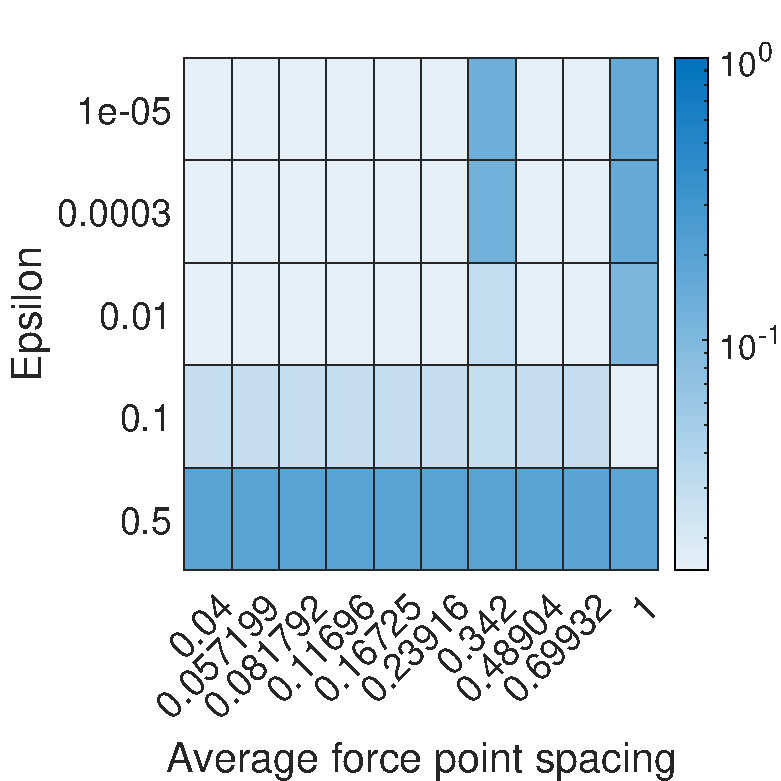
\includegraphics[width=0.4\textwidth]{Images/Hybrid/DisjointFMM.pdf}}\hfill
 \subfloat[\label{fig:JOINFMM}]{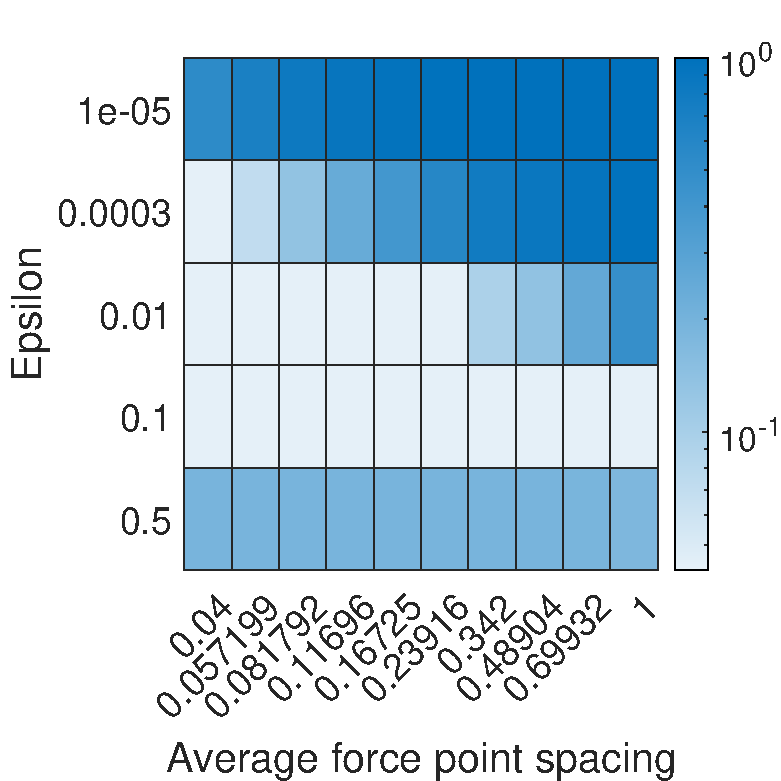
\includegraphics[width=0.4\textwidth]{Images/Hybrid/IntersectingFMM.pdf}}
 \caption[The relative error in calculating the grand resistance matrix for the unit sphere using Nyström and NEAREST when calculated through the KIFMM method.]{The relative error in calculating the grand resistance matrix for the unit sphere using Nyström and NEAREST when calculated through the KIFMM method. (i) Relative error in Grand Residence matrix for the disjoint case of the hybrid NEAREST KIFMM method. (ii) Relative error in Grand Residence matrix for the contained case of the hybrid NEAREST KIFMM method.}
 \label{fig:NEARESTCOMPFMM}
\end{figure}